\begin{figure}
	\centering
	\label{fig:pendulum}
	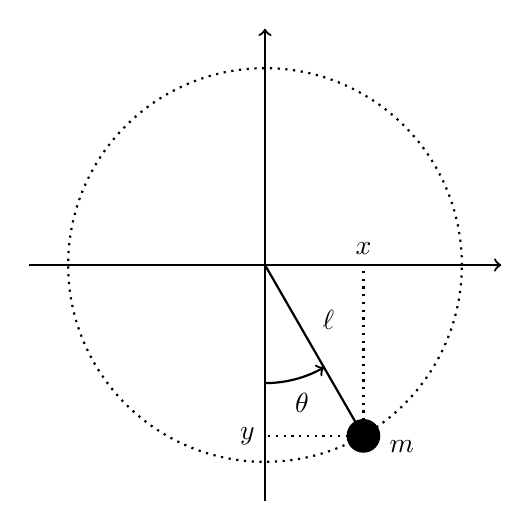
\begin{tikzpicture}[thick]
		\draw [<->,thick] (0,3) |- (3,0);
		\draw [-] (0,-3) |- (-3,0);
		\draw [thick] (0,0) -- (1.25, -2.17);
		
		\draw [dotted,thick] (1.25, -2.17) -- (0, -2.17);
		\draw [dotted,thick] (1.25, -2.17) -- (1.25,0);
		
		\draw [dotted,color=black] circle(2.5);
		\draw [fill = black] (1.25,-2.17) circle [radius=0.2];
		\draw[->] (0,-1.5) arc (-90:-60:1.5) ;
		
		\node [right] at (1.45,-2.3) {$m$};
		\node [right] at (0.6,-0.7) {$\ell$};
		\node [right] at (0.25,-1.75) {$\theta$};
		\node [left] at (0, -2.17) {$y$};
		\node [above] at (1.25,0) {$x$};
	\end{tikzpicture}
	\caption{A simple pendulum.}
\end{figure}
